\documentclass[12pt, openany]{book}

% This is all the packages and settings and so on.
% It is using custom fonts that needs to be installed on the computer. If they are not present, they have to be added manually.
\usepackage[
	citestyle=ieee, 
    bibstyle=ieee,
    style=numeric-comp,
    sorting=nty,
    maxbibnames=99, % Make sure we are printing all authors in the appendix
    ]{biblatex}
    
% Makes the last name first in the bibliography.
% \DeclareNameAlias{author}{last-first}
\DeclareNameAlias{author}{family-given}
    
% Specify the margins. This is 6.25inches in text with which 
% can be used to size figures to the correct size.
\usepackage[a4paper, margin=2.5625cm]{geometry}

\usepackage{eso-pic}					% Packages for layout and graphics 
\usepackage{graphicx}
\usepackage{tikz}
\usetikzlibrary{fadings}
\usepackage{setspace}
% \usepackage{tocloft}		 			% Fixing a bug with page style changes for toc
% \tocloftpagestyle{plain}
\usepackage{etoc} 						% Separate tocs for appendix and the rest    
\usepackage{chngcntr}					% Count figures within chapters
\usepackage{booktabs}					% Table formatting
\usepackage{fancyhdr}					% Setting the style for header and footer.
\usepackage{tabularx}
\usepackage{multirow}                   % For better tables 
\usepackage{nameref}					% References with names
\usepackage[parfill]{parskip}			% New line instead of indent for sections
\usepackage{tcolorbox}					% Create boxes around content
\tcbset{colback=white,arc=0mm}

\usepackage{amsmath}
\usepackage{mathdots}
\usepackage{yhmath}
\usepackage{siunitx}
\usepackage{array}
\usepackage{gensymb}
\usepackage{amssymb}
\usepackage{mathtools}              % Add text to math arrows.

\usepackage{cancel}
\usepackage{color}
\usepackage{multirow}
\usepackage{textcomp}               % Fixing warning for gensyb \perthousand
\usepackage{svg}                    % including svg files
%\usepackage{caption}                % For subfigures
%\usepackage{subcaption}
\usepackage{subfigure}
\usepackage{fontspec}
\usepackage{sectsty}
\usepackage{subfigure}
\usepackage[subfigure]{tocloft}

\usepackage[printonlyused]{acronym}
\usepackage[hidelinks]{hyperref}		% Clickable links


\counterwithin{figure}{section} 
\counterwithin{table}{section}

% Specifying fonts
\setmainfont{Georgia} 
\setsansfont{Arial}
\newfontfamily\footerfont{Georgia}

\chapterfont{\sffamily\fontsize{17}{17}}
\sectionfont{\sffamily\fontsize{14}{15}}
\subsectionfont{\sffamily\fontsize{13}{15}}
\subsubsectionfont{\sffamily\fontsize{12}{15}}

% Remove the title and make sure that the text is adjusted
% \usepackage{abstract}
% \setlength{\absleftindent}{0mm}
% \renewcommand{\abstractname}{\vspace{-\baselineskip}}
% \renewcommand{\abstractnamefont}{\sffamily\fontsize{14}{15}}
% \renewcommand{\abstracttextfont}{\normalfont\fontsize{12}{13}}

% Renaming and setting style of table of contents
\renewcommand*\contentsname{Contents}
\renewcommand*\cfttoctitlefont{\fontsize{16}{0}\bf\sffamily}
\renewcommand\cftchapfont{\fontsize{14}{0}\bf\sffamily}
\renewcommand\cftchappagefont{\fontsize{13}{0}\bf\sffamily}
\renewcommand\cftsecfont{\fontsize{12}{0}\sffamily}
\renewcommand\cftsecpagefont{\fontsize{12}{0}\sffamily}
\renewcommand\cftsubsecfont{\fontsize{12}{0}\sffamily}
\renewcommand\cftsubsecpagefont{\fontsize{12}{0}\sffamily}

% Styling the header and footer
\fancyhf{}
\fancyhead{}
\fancyfoot{}
\fancyhead[L]{\fontsize{11}{10}\selectfont\leftmark}
\fancyfoot[R]{\footerfont\thepage}
\setlength{\headheight}{15.5pt}


\fancypagestyle{plain}{
    \fancyhf{}
    \fancyhead{}
    \fancyfoot{}
    \renewcommand{\headrulewidth}{0pt}
    \fancyfoot[R]{\footerfont\thepage}
}

\pagestyle{fancy}

% Making the command for placing text in random locations
\newcommand\PlaceText[3]{%
\begin{tikzpicture}[remember picture,overlay]
\node[outer sep=0pt,inner sep=0pt,anchor=south west] 
  at ([xshift=#1,yshift=-#2]current page.north west) {#3};
\end{tikzpicture}%
}

% Disable hyphenation
\pretolerance=10000
\tolerance=2000 
\emergencystretch=50pt


% Defining files for bibliography
%\addbibresource{ref.bib}
\addbibresource{references.bib}
% Add a second bibliography file for the second author to allow
% both to update it through the mendeley integration.
% \addbibresource{ref-author-2.bib}

% Defining document information
\title{An eQTL-based analysis for investigation of kidney cancer risk loci in a Japanese cohort}
\newcommand{\subtitle}{KTH Master Thesis Report}
\author{Xiya Song}
\usepackage{graphicx}
% \usepackage{hyperref}
\hypersetup{hidelinks,
	colorlinks=true,
	allcolors=black,
	pdfstartview=Fit,
	breaklinks=true}
\graphicspath{ {./figures/} }

\begin{document}
\setstretch{1.4}

% The front page of the document
\pagenumbering{roman}
\makeatletter
\begin{titlepage}

\vspace*{-4.6\baselineskip}
\hspace*{-0.15\textwidth}
\includegraphics[width=0.2\paperwidth]{setup/img/kth-logo.jpg}
\par\vspace*{2.5\baselineskip}

\PlaceText{65mm}{12mm}{\fontsize{12}{0}\sffamily DEGREE PROJECT IN TECHNOLOGY,}
\PlaceText{65mm}{17mm}{\fontsize{12}{0}\sffamily SECOND CYCLE, 30 CREDITS}
\PlaceText{65mm}{22mm}{\fontsize{12}{0}\sffamily\itshape STOCKHOLM, SWEDEN \the\year}

~\\

\makebox[0pt][l]{%
\begin{minipage}[b]{0.25\textwidth}
~\\
\end{minipage}
\begin{minipage}{0.65\textwidth}
\begin{flushleft}
{\fontsize{28}{24}\bf\sffamily\@title\\}
\vspace{1cm}
{\fontsize{19}{17}\bf\sffamily \subtitle\\}
\vspace{1cm} 
{\fontsize{16}{18}\sffamily \@author}\\
\end{flushleft}
\end{minipage}
}


% \hspace*{-3cm}\begin{minipage}[b]{63.5mm}
% ~\\
% \end{minipage}
% \begin{minipage}{0.65\textwidth}
% \begin{flushleft}
% {\fontsize{28}{24}\bf\sffamily\@title\\}
% \vspace{0.5cm}
% {\fontsize{19}{17}\bf\sffamily \subtitle\\}
% \vspace{0.5cm} 
% {\fontsize{16}{0}\sffamily \@author}\\
% \end{flushleft}
% \end{minipage}


\AddToShipoutPictureBG*{%]
    \AtPageLowerLeft{%
        
\includegraphics[width=1.0\paperwidth]{setup/img/kth-footer.png}
    }%
}

\PlaceText{70mm}{280mm}{\color{white}\fontsize{12}{0}\sffamily KTH ROYAL INSTITUTE OF TECHNOLOGY }
%\PlaceText{70mm}{285mm}{\color{white}\fontsize{8}{0}\sffamily xxx falculty  }
\end{titlepage}
\makeatother

\newpage
\newpage
\thispagestyle{plain}
~\\
\vfill
{ \setstretch{1.1}
	\subsection*{Authors}
	Author Name: Xiya Song\\
	Molecular Techniques In Life Science\\
	KTH Royal Institute of Technology
	
	\subsection*{Place for Project}
	Stockholm, Sweden\\
	
	\subsection*{Supervisor }
	The Supervisor: Dr.Cheng Zhang\\
	Principal investigator: Professor Adil Mardinoglu \\
	Place: Stockholm, Sweden \\
	KTH Royal Institute of Technology
	~
}


\newpage
\thispagestyle{plain}
%%%%%%%%%%%%%%%%%%%%%%%%%%%%%%%%%%%%
%%  The English abstract          %%
%%%%%%%%%%%%%%%%%%%%%%%%%%%%%%%%%%%%
\chapter*{Abstract}
%%%%%%%%%%%%%%%%%%%%%%%%%%%%%%%%%%%%

Clear cell renal cell carcinoma (ccRCC) is the most common form of kidney cancer in adults. Further investigation of the molecular mechanisms and underlying processes of ccRCC is crucial for targeted drug development. Expression quantitative trait loci (eQTL) analysis is a method to identify genetic variants that might affect gene expression. The identified eQTLs and genes being regulated (eGenes) from tumor tissue provide valuable information concerning cancer development. In this study, the DNA-sequencing and RNA-sequencing data of 100 Japanese ccRCC patients were used to perform an eQTL analysis using the methodology developed by the Genotype-Tissue Expression (GTEx) project. A list of 805 significant eGenes with corresponding most significant eQTLs has been identified for the Japanese ccRCC cohort. Compared to the healthy kidney eQTLs database in the GTEx database, there are 518 new eGenes that were only discovered in the Japanese cancer cohort. Furthermore, 13 new eGenes are associated with recurrently mutated somatic sites, indicating that they may be driver genes in cancer development. The long non-coding RNA (lncRNA) genes and the Ubiquitin-specific protease (USPs) family have shown an important role in ccRCC based on the results. In summary, the study provides a comprehensive database of the eGenes and eQTLs specific to Japanese ccRCC patients and identified some key genes as potential drug targets.

\subsection*{Keywords}
eQTLs, eGenes, clear cell renal carcinoma(ccRCC),GTEx, kidney cancer, somatic mutations

\newpage
\thispagestyle{plain}
\chapter*{Acknowledgements}

I would like to express my gratitude to all those who helped me during the writing of this thesis. First of all, I want to thank my supervisor, Dr.Cheng Zhang, for his continuous encouragement and guidance during the period of this project. Also, he has provided me the ground idea of the whole research and all the resources needed in this degree project. I am also greatly indebted to professor Adil Mardinoglu who gave me the opportunity to enter the sysmedicine lab. I am also very grateful to all the Ph.D students and postdocs researcher in the lab, who gave me kindly advice and warming help, especially for Dr.Xiangyu Li who helped me with handling specific details during the project, and Ph.D student Hong Yang who gave me the help on software installation and other tough obstacles. I also want to thank all the teachers and my classmates in this two-year's master study who gave me a great study experience. Last my thanks would go to my beloved family for their loving considerations and great confidence in me all through these years.


\newpage

\etocdepthtag.toc{mtchapter}
\etocsettagdepth{mtchapter}{subsection}
\etocsettagdepth{mtappendix}{none}
\thispagestyle{plain}
\tableofcontents

\newpage




\pagenumbering{arabic}

\chapter{Introduction}

\section{Background}
\label{sec:background}

\subsection{Clear cell renal cell carcinoma(ccRCC)}
\label{subsec:Clear}

Renal cell carcinoma (RCC) makes up approximately 80\% of kidney cancer, and it is the seventh most common cancer in men and the ninth most common cancer in women\cite{rini_renal_2009}. RCC is thought to originate from cells in the proximal convoluted tubule of the nephron. A subtype named clear cell renal cell carcinoma (ccRCC) is the most common and aggressive form of RCC and we have little knowledge of the related tumor suppressor genes or oncogenes\cite{yang_gene_2017}. The surgical excision of the tumor or the whole kidney is a major approach to cure patients but it is not only limited by patients’condition but also kills the kidney function and has risk factors for recurrence after surgery. As a result, we need to investigate the underlying molecular mechanisms of ccRCC to develop potential targeted therapy.

Previous research shows that ccRCC is mostly characterized by the Von Hippel-Lindau (VHL) tumor suppressor gene mutation. VHL gene encodes the proteion pVHL, a recognition component of an E3-ubiquitin ligase complex. This complex targets hypoxia-inducible factor(HIF)-1α and HIF-2α for proteasomal degradation under normoxic conditions. The loss of the VHL gene function results in abnormal activation of HIF factors that participate in the glycolysis, angiogenesis and metastasis processes of tumor cells. However, the loss of VHL gene function alone is not sufficient to develop ccRCC\cite{sanchez_genetic_2018}. Another 3 chromatin modifying enzyme genes BAP1, PBRM1, and SETD2 are also frequently mutated in ccRCC based on the Cancer Genome Atlas (TCGA) data\cite{eckel-passow_8q24_2020}. There is also evidence that the PI3K / AKT / mTOR pathway contributes significantly to ccRCC prognosis. This pathway is typically regulated by other factors, such as miRNAs\cite{braga_molecular_2019}. Previous studies have also emphasized the important regulatory roles of long non-coding RNAs(lncRNAs)\cite{zeng_prognosis_2019} in ccRCC developments. However, ccRCC is a highly heterogeneous disease and the information available at this time is insufficient to provide a clear picture of the initiation and progression of the disease. The development of ccRCC can be linked to combinations of alterations at different levels, such as inactivation or abnormal expression levels of proteins, as well as alterations in regulatory elements, transcription factors involved in key pathways. Notably, nearly all those alterations are originally started by genetic mutations. Not only the ccRCC, but also other cancers are mostly driven by DNA-level variations. As a result, it is important to explore the cancers development that start at the DNA level.


\subsection{The aim of GWAS studies and eQTL analysis}

As the reason mentioned at the end of section \ref{subsec:Clear}, the research methods such as Genome-wide association studies (GWAS) have contributed to the discovery of disease-related genetic variations. The GWAS studies aim at scanning the genomes of populations to discover genetic markers that are used as predictors of a certain trait or disease. However, most of the identified single-nucleotide polymorphisms (SNPs) from GWAS studies fall within the non-coding region, which means they might only function as indirectly regulatory factors. The GWAS study uses a variety of diseases and traits as phenotypes, so GWAS ‘hit’ does not necessarily identify the gene, tissue, cell, or mechanism that mediates the direct biological effect\cite{sampson_glomerular_2019}. As a result, they cannot provide information about genes and pathways that directly relate to the risk loci.
 
The expression quantitative trait loci (eQTL) analysis is aiming at finding genetic variations (both SNPs or Indels) that directly control gene expression. It could be explained as a special genome-wide association study (GWAS) that uses quantitative gene expression levels as phenotypes. The figure \ref{Causal} is a nice illustration of relationship between GWAS and eQTL analysis. By performing eQTL analysis, it is possible to uncover genetic variants that regulate gene expression and construct gene regulatory networks. The eGenes, defined as genes that have at least one significant eQTL site, will provide a reference for driver disease genes identification. The eQTL analysis has been used in several relevant studies to explore the oncogenic mutation, risk loci, and pathway alterations in ccRCC. The eQTL study will connect mutations found in ccRCC patients with known gene regulation mechanisms, and also will open the possibility of uncovering novel mechanisms.

\begin{figure}[h]
\centering
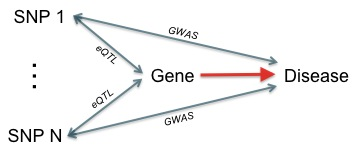
\includegraphics[width=0.5\textwidth]{figures/Causal.jpg}
\caption{A simple illustration for the relationship of SNPs,eQTLs,gene,GWAS and diseases(http://sherlock.ucsf.edu/).}
\label{Causal}
\end{figure}

\subsection{Existed healthy kidney eQTL analysis from GTEx using software FastQTL}

In recent years, eQTL-related databases and statistical methods have both been developed. The Genotype-Tissue Expression (GTEx) project includes eQTL analysis data on 54 non-disease tissues from 948 donors with over 15000 samples collected. In the GTEx version 8 release, there are 73 kidney-cortex samples with donor genotype information. The software packages which implement statistical methods of eQTL analysis for single tissue or single cell type are now relatively mature, such as Matrix eQTL\cite{shabalin_matrix_2012} and FastQTL\cite{ongen_fast_2016} improved based on Matrix eQTL. The latest GTEx cis eQTL mapping was performed using FastQTL.

In the GTEx portal((https://gtexportal.org/home/), the donor's kidney cortex tissues were collected and the eQTLs were analyzed using 73 samples. The donors usually died because of traumatic injury, cerebrovascular or heart disease, etc. Few of them have diseases related to the renal. This study provided a background of potential key genetic variations that regulate the kidney tissue's gene expression in the donor bodies but did not contribute to the landscape of specific diseases, such as ccRCC. This study majorly included White(84.6\%) subjects, followed by African American(12.9\%) ones, and only a small proportion of Asian(1.3\%) subjects were involved. As a result, there is also a lack of Asian targeted eQTLs in the GTEx database.

\subsection{Variants type appeared in cancer tissues}
\label{subsec:Variants type appeared in cancer tissues}

A lot of published cancer-related eQTL analyses have been published. Gene expression regulation in tumors is largely different from healthy tissue. Firstly, the tumor tissues usually carry lots of somatic mutations. The somatic mutations are not inherited by parents, but occur when cancer cells are developing. The somatic mutations could act either as "driver" mutations that are oncogenic or "passenger" mutations that promote the tumor lesions. The various types of mutations that appeared in cancer cells could be copy number variations, SNPs, Indels, and also epigenetic changes such as DNA methylation. The "driver" mutations bring growth advantage to the tumor cells and usually act as non-synonymous mutations in coding exons, and the "driver" genes are usually identified as protein kinase family\cite{greenman_patterns_2007}.

Besides, gene expression could also be affected by germline variants. Germline variants are usually applied to predict some inherited cancer's developing risks or assess drug sensitivity and toxicity for specific patients. Notably, the germline variants have been identified to have associations with cancer gene expression from a lot of studies such as a pan-cancer study in USA\cite{huang_pathogenic_2018} that identified the pathogenic germline mutations.

SNPs in different genome locations affect gene expression in different ways. SNPs within transcriptional regulatory elements might alter transcription efficiency, and SNPs within genes might change the mRNA splicing and mRNA stability to affect the detected transcripts and downstream translation(Robert and Pelletier, 2018). Some SNPs might regulate genes on larger distances and even different chromosomes. Most eQTL analyses focus on finding the cis-eQTLs that the SNPs act on local genes because the trans-eQTLs that act on distant genes tend to have weaker effects than cis-eQTLs and the detection requires a larger sample size and more calculations\cite{shan_identification_2019}.


\section{Methodology}

The variations in two different levels(germline level and somatic level) described in \ref{subsec:Variants type appeared in cancer tissues} brings the difficulties in cancer-related eQTLs analysis. In a research about breast cancer eQTLs\cite{li_integrative_2013}, the influence of somatic copy number variations and the DNA methylation was first considered in a multivariate linear model and the residual expression was regressed to the germline genotypes in order to find the germline risk loci. This model is able to assess the influence of 3 kinds of variations separately, however, it also needs additional data collection and processing for DNA methylation and copy number variations. A research about colon cancer eQTLs\cite{moreno_colon-specific_2018} has pointed out that the expression of genes in tumor tissues has changed greatly compared to normal, so the expression value from normal tissues was majorly used. The genotypes used in the colon study were from both adjacent normal colon tissues(obtained from cancer patients) and normal colon tissues(obtained from healthy volunteers). However, in this degree project, the gene expression of normal tissues was not available. In able to identify eQTLs in tumor tissues, several studies were focused on the somatic mutations inside the tumor samples. A research including multiple tumor types\cite{zhang_global_2018} was aimed at identifying somatic mutated "loci" in tumor samples that affect tumor gene expressions. They performed whole-genome sequencing for 930 tumors and grouped the mutations that close to each other within 50 bps into recurrently mutated loci. To achieve this union of adjacent mutations, huge sample size and deep sequencing depth were needed. 

The research about eQTLs in ccRCC diseases is relatively rare. A research\cite{yang_gene_2017} used the whole-exome sequencing data from 417 paired tumor and normal samples to get the somatic mutations. Then they used differential expressed gene modules to process the eQTL analysis, which generated from RNA-sequencing data from both tumor and normal tissues. 


\section{Goals}

This project’s main goal is to comprehensively understand the gene expression determinants in ccRCC and gain insights into the underlying biology of ccRCC development. In this study, existing sequencing data from the other research project are used, but are analyzed in a different manner. The eQTL analysis based on the provided ccRCC cancer cohort will able to give the information of SNPs that significantly affects the cancer tissue's gene expression. Furthermore, the eGenes that show high expression changes controlled by genotypes will reflect potential cancer-related cellular pathways. The unique population composition of this cohort will give more reference to Asia-specific ccRCC eQTLs. By comparing the identified kidney cancer eGenes with GTEx healthy kidney databases, special cancer-related eQTLs and eGenes are able to be discovered. This information will replenish current kidney tissue disease databases and provide potential strategies for drug development.
\chapter{Materials and methods}
% \thispagestyle{fancy}

Based on the former literature review, the technical route of this degree project was designed as the flow chart showed in Figure \ref{flow-chart}. In the eQTL analysis, the genotypes and gene expression of the tumor tissue were used. The somatic mutations were also identified using DNA sequencing data from both tumor tissues and matched normal tissues. The overlapped genes between somatically mutated genes and the eGenes identified through eQTL analysis were defined as potential driver eGenes that hold higher potential for triggering cancer development. After excluding the overlapped eGenes between the GTEx portal and this study, the eGenes specific to this Japanese cancer cohort can be identified.


\begin{figure}[h]
\centering
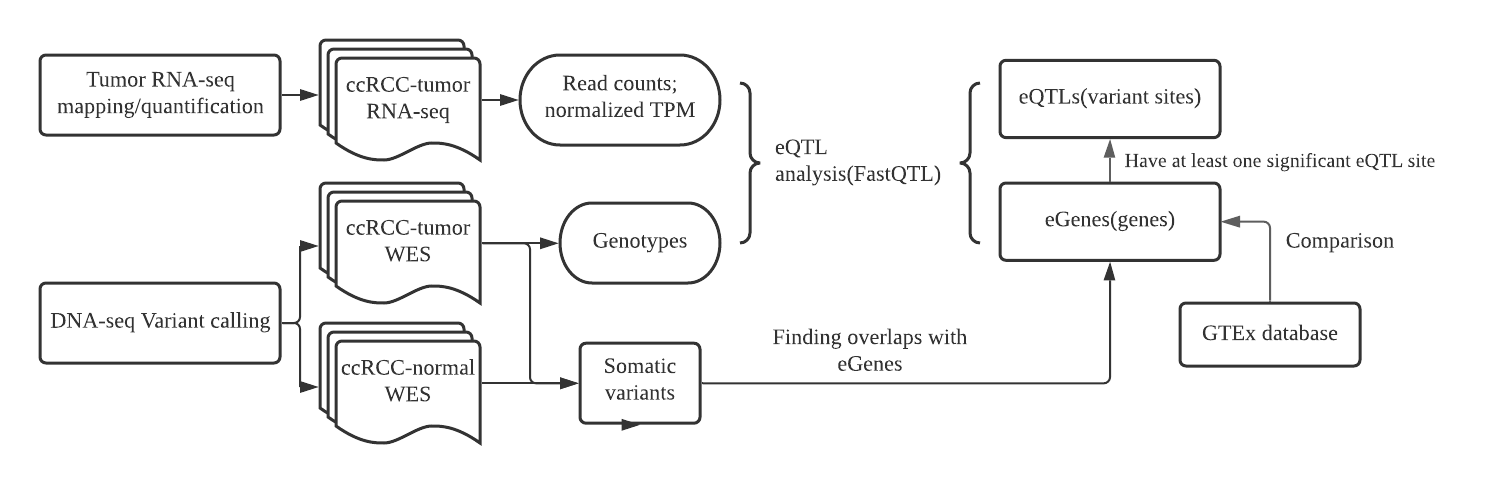
\includegraphics[width=1.0\textwidth]{figures/eQTL-analysis (3).png}
\caption{Study flow in this degree project}
\label{flow-chart}
\end{figure}

This project used both DNA-sequencing and RNA-sequencing data from 100 ccRCC patients from Asia(Japan), which originated from an integrated research from Japan\cite{sato_integrated_2013}. All the sequence data were in bam format and downloaded from the European genome-phenome archive, coded with EGAD00001000597.The DNA-sequencing data contains tumor data from ccRCC tumor specimens and matched normal data from either normal kidney tissue(97 patients) or peripheral blood(3 patients). The DNA-sequencing used SureSelect targeted sequencing which performed by Illumina HiSeq 2000 platform with 100-bp paired-end reads. Based on the original dataset description, the mean depths of coverage of the entire targeted regions were 129×. The RNA-sequencing was performed on the same platform for 100 ccRCC cases. The data analysis was handled mostly by Uppmax platform and some by Docker images provided by GTEx.\\

The cohort consists of 23 females and 77 males and the ages are widely distributed between 35 to 91. The patient's condition was recorded in the metadata, majorly includes the stage at diagnosis, Fuhrman grade, metastases, and outcome(dead/alive). Some metadata were used in generating covariates in eQTL analysis.

See the table \ref{tab:sample-table} for a summary of used data set.

\begin{table}[!ht]
\centering
\caption{A summary of dataset used in this project}
~\\
\label{tab:sample-table}
\begin{tabular}{lll}
\toprule
\textbf{SAMPLE}		  &\textbf{Sequencing method}	& \textbf{Amount}                                                                                                                                                  \\ \toprule
ccRCC Tumor                &Whole exome sequencing  & 100 \\
\midrule
ccRCC Normal 	& Whole exome sequencing & 100 \\
\midrule
ccRCC Tumor         & RNA-sequencing        & 100\\
\bottomrule
\end{tabular}
\end{table}



\section{RNA-sequencing and quantification}

The processing of RNA-sequencing data followed the GTEx portal with some parameter adjustment based on the ccRCC dataset.

The index for STAR(v2.5.3a)\cite{dobin_star_2013} was built with matched sequencing read length 100bp. The genome file GRCh38/hg38 and the annotation file GENCODE v26 was used.The downloaded BAM files were transformed to paired fastq files using Picard(http://broadinstitute.github.io/picard/)function SamToFastq. The FASTQ format paired-files were aligned to GRCh38/hg38 reference genome using STAR(v2.5.3a) \cite{dobin_star_2013}. STAR were set to two-pass mode and the results have been sorted by coordinate using samtools(http://www.htslib.org/). The duplicates were removed using Picard function MarkDuplicates.The gene-level quantification was generated use RNA-SeQC2.3.6(https://github.com/getzlab/rnaseqc). During the process, the read-level filters were applied automatically by RNA-SeQC to ensure well quantification. The RNA-seq data were performed by unstrand-specific sequencing. The related collapsed-gene model that combined all isoforms of a gene into a single transcript was used as an input file for RNA-SeQC. The file is available in GTEx resources(https://console.cloud.google.com/storage/browser/gtex-resources/GENCODE). The outputs for 100 samples were combined into one union file and prepared for eQTL analysis.


\section{DNA-sequencing processing and mutations calling}

The processing pipeline of DNA-sequencing data was based on The Genome Analysis Toolkit (GATK) 4.1.1.0\cite{mckenna_genome_2010}'s best practice. Several details have been adjusted using GTEx published literature\cite{noauthor_gtex_2020}'s supplementary materials as a guide.


\subsection{Pre-processing for variant discovery} 
In this step, the raw bam files were all converted into FASTQ files and re-mapped to hg38 using BWA-MEM. The read group information was added using Picard. In order to improve the quality of variant calling, local realignment (using GATK IndelRealigner) was applied first. The GATK's duplicates removal and base quality score recalibration were then applied to all the 200 BAM files.

\subsection{Variants calling on tumor samples} 
GATK HaplotypeCaller was applied to call all the appeared variants (SNVs, Indels) from each tumor sample. The variants for 100 samples were joint-called using GATK GenomicsDBImport and GenotypeGVCFs. The variants were restricted to chromosomes 1-22 and chromosome X. 

\subsection{Variants quality control}
The variants were filtered based on multiple steps listed below. 

1)Variant (Quality Score) Recalibration (VQSR) with allele-specific mode. This mode took consideration of multi-allelic sites. Before VQSR, a hard filter for Excess heterozygosity(ExcessHet) > 54.69 was applied considering a relativey large cohort size(100). The VQSR step calculated a model using machine learning and applied a threshold of 99.8\% (for SNPs) and 99.95\%(for Indels) to filter the variants.

2)Applied hard-filtering at site-level. Firstly, the sites with QUAL <30 or QualByDepth(QD) <2.0 threshold were filtered out. As an explaination, QUAL value is the Phred-scaled quality score and QD is the QUAL score normalized by Depth. Then the sites with low Inbreed Coefficient < -0.3 were filtered out. An Inbreed Coefficient value of 0 means that the site is in Hardy-Weinberg equilibrium. But negative value indicating that the sites were with bad mapping. The value of -0.3 was chosen to align with GTEx.

3) For filtration at the genotype level, the sum VCF file of 100 samples was processed through the GATK genotype refinement pipeline to re-calculate the GQ value per sample at per variant site. The variants from the 1000 Genomes project were used as a supporting file. The genotypes with re-calculated GQ <20 or the minimum read depth (DP) <3 were filtered using GATK VariantFiltration. After this filtration, the total variant sites were not changed but the unqualified genotypes were all set to missing(shown as "./.")

4) In order to continue downstream quality control, the multi-allelic sites were split into biallelic sites using Hail 0.2 (https://hail.is/).

5) After splitting, the monomorphic SNPs that have no called alternative alleles (AC==0) were removed using bcftools(https://samtools.github.io/bcftools/)filter. AC is the allele count in genotypes for the “ALT” allele(s).

6) The missingness of genotypes at each site was set to the maximum tolerance of 0.25, which means only the variant sites that called in more than 75\%  of individuals were kept. This step used bcftools for filtration and it ensured convincing genotype results to be used in eQTL analysis. The threshold is less strict than the threshold that GTEx used (0.15), but still filtered out most of the variants.

7) The threshold of minor allele frequencies (MAF) was set to <= 0.01 using bcftools , which means a variant site was excluded if its minor allele is found in equal or less than 1\% genotypes. 

See Table \ref{tab:Mutation_filter_step} for a detailed number of variants in different filtering process.
\begin{table}[!ht]
\centering
\caption{Variants QC filtering from Haplotypecaller}
~\\
\label{tab:Mutation_filter_step}
\begin{tabular}{lll}
\toprule
\textbf{Filtering / processing criterion}		  & \textbf{Total sites}   &\textbf{Percentage}                                                                                                                                       \\ \toprule
Initial variants                   & 7088610	&100.00\%	\\
\midrule
VQSR and ExcessHet not PASS & 6813720 	&96.12\%	\\
\midrule
QD <2.0 or QUAL <30 & 6804941	&96.00\%	\\
\midrule
InbreedingCoeff < -0.3  & 6802902	&95.97\%	\\
\midrule
Hail splitting Multi-allelic sites 	& 6927794 	&\\
\midrule
Monomorphic sites with AC =0 & 6356484	&89.67\% \\
\midrule
Missingness > 25\% & 459062	&6.48\% \\
\midrule
MAF <=1\% & 284774	& 4.02\% \\ 
\bottomrule
\end{tabular}
\end{table}


\subsection{Somatic mutations identification using tumor samples and matched normal}
The GATK Mutect2 was applied to prepared tumor BAM files and matched normal BAM files to identify somatic variants. While using the 'Tumor with matched normal' model, a panel of normal(PON) file provided by GATK was also used to filter the germline variants. FilterMutectCalls was used to filter the somatic mutations which considered read orientation bias and cross-contamination.\\

\subsection{Mutations annotation}

The mutation files were first annotated using GATK VariantAnnotator using dbsnp138 databases. Then the SnpEff\cite{cingolani_program_2012}(http://pcingola.github.io/SnpEff/) was used for a detailed functional annotation.

\section{Japanese cohort eQTL analysis}

The mapping strategy in FastQTL is based on linear regression. For a simple linear regression, the gene expression is the response variable while only genotypes of each sample are included as explanatory variables that affect the value of gene expression. The formula is as follows: $$ Y_i=\beta_0+\beta x_i+\epsilon_i $$

The multiple linear regression uses several explanatory variables to predict the outcome of response variable, which make it possible to consider other possible factors such as sex, gender and other types of independent variables. Those factors could input as covariates when perform linear regression using FastQTL.The formula is as follows:$$ Y_i=\beta_0+\beta_1 x_{i1}+\beta_2 x_{i2}+ ... + \beta_p x_{ip}+\epsilon_i $$  

In the two formulas,  $Y_i $ represents the gene expression, and $x_i$ represents all the factors that might regulate the gene expression, including genotypes and covariates of each sample.

When testing the associations between genes and variants, for a single gene, there are series of variants inside the cis window (Within 1 Megabase for both upstream and downstream from the transcription start site). Millions of association tests were used to scan all the phenotype-variant pairs, which is called a 'norminal pass' in FastQTL. Due to the large amounts of tests performed, a multiple testing correction is needed to assess the significance of candidate variants. The correction is achieved by analyzing a range of permuted datasets per phenotype, which is called a 'permutation pass' in FastQTL.

To perform the eQTL analysis using software FastQTL\cite{ongen_fast_2016}, several steps were used for preparation. The environment was prepared based on a Docker image provided by GTEx.The gene-level expression data for 100 patients were normalized based on the same principle with GTEx.The sample id appeared in DNA-sequencing and RNA-sequencing for the same individual was mapped in a list as a reference for eQTL mapping. A cis-mapping windows range was set to within 1Mb between variants and genes.The variant IDs were set using variants information(chromosome, position,REF,ALT). An adaptive permutation pass between 100 to 1000 times was used to get the adjusted p-value for each site.The missing genotypes were imputed when FastQTL starts to read the genotype data file. Extra gene and variant information were added to the final eQTL results.

\subsection{Covariates generation}
Covariates that combined in different aspects were used in FastQTL. In order to estimate hidden determinants of gene expression, the probabilistic estimation of expression residuals (PEER)\cite{stegle_using_2012}were used. The number of PEER factors(15) was set based on the sample size(100). Usually, the top 5 PC components from PCA analysis across all the filtered genotypes were used for population stratification. All the samples from the Japanese cohort theoretically have the same genetic ancestry. Nevertheless, the first 5 PCs calculated using PLINKv1.9\cite{purcell_plink_2007} were still included in the covariates file. The sex and age factor(below 50 years old or above) were considered as part of covariates. Finally, the patient's stage of diagnosis which recorded by the metadata was included as covariates in the following rules:  the information of tumor size(T) has been encoded as numbers from 1 to 4; whether cancer has spread into nodes(N) or not has been encoded as numbers 0,1 or 2(represents an extent of spread);  whether cancer has spread to distant tissues, named metastasis situation (M)  and has been encoded as 0 or 1. The FastQTL was run by both nominal-pass and permutation-pass. A minor allele sample count threshold of at least 10 samples was set when running FastQTL.

\subsection{Gene set enrichment analysis}

The gene set enrichment analysis for a list of significant eGenes was achieved by the web-based tool Enrichr\cite{kuleshov_enrichr_2016} with default setting. 

\section{GTEx kidney tissue eQTLs data acquision}

The eQTLs analysis results (V8 release) for all the tissues are available at GTEx portal(https://www.gtexportal.org/home/datasets).The kidney tissue-specific eQTL data were downloaded and extracted for downstream comparison. In order to obtain a list of significant eGenes, only eGenes with a q value lower than 0.05 were collected.

\section{Boxplot of eQTLs and eGenes}

The boxplot that described how the genotype affects corresponding gene expression for Japanese cohort results was drawn using an R script provided in appendices\ref{sec:Appendices}. The genotypes have been transformed using following rules: The genotypes with 0/0 were changed to value 0; the genotypes with 0/1 were changed to value 1; the genotypes with 1/1 were changed  to value 2. The missing genotypes with ./. were set to value 0. 


\chapter{Results}

\section{PCA analysis of population genetics}
Based on the Principal component analysis(PCA)of 100 patients genotype information, there were no significant principal component.components.  The principal component 1 (PC1) and PC2 explained nearly the same percentage (20.17\% and 20.1\%, respectively) of genotype variation. As the methods part mentioned, the first 5 PCs were used as covariates for eQTL mapping.

\textbf{
\begin{figure}[h]
\centering
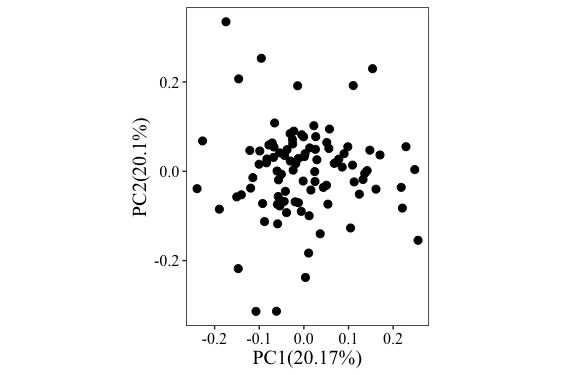
\includegraphics[width=0.8\textwidth]{figures/pca.png}
\caption{The figure illustrates the PCA plot for genotypes for 100 Japanese patients. The PC1 and PC2 are displayed on the x-axis and y-axis, respectively.}
\end{figure}
}
\section{Tumor tissue total variants}
A total of 284774 variants were called in Japanese ccRCC cohort tumor samples, including 244803 SNPs, 17346 insertions, and 22625 deletions. There were 0.182\% of variants annotated with a ‘HIGH’ impact, which means that the variant causes deleterious gene effects as determined by SnpEff. Similarly, nonsense mutations only accounted for 0.366\% of all mutations. Most of the mutations belong to missense(47.19\%) and silent mutations(52.445\%). The Transition/Transversion ratio was 2.37. As for the location of the mutations, the majority of mutations were found in introns (53.19\%). The percentage of exonic mutations is 13.24\%.The mutations also appeared in the upstream and downstream regions which occupied 12.34\% and 16.51\% , respectively.

\section{Somatic mutations in the Japanese cohort}

Only mutations remained after running FilterMutectCalls were used for statistics and downstream analysis. A total of 23997 somatic variants were remained, including 21046 SNPs,352 Multiple-nucleotide polymorphism(MNPs),610 insertions, and 1989 deletions. Variants with ‘HIGH’ impact represent 2.32\% of total somatic mutations. Missense mutations accounted for a greater proportion of the mutations (71.281\%) than silent mutations (24.753\%). The somatic mutation load in 100 patients was shown in Figure\ref{Somatic_load}. Most of the patients have around 250 to 400 somatic variants which are log-transformed to 2.4-2.6. A total of 712 mutated genes with at least five recurrent mutations have been identified. BAGE2, a long non-coding RNA (lncRNA) gene often related to melanoma, had the highest frequency of somatic mutations (67 times). The second most frequent mutated gene was VHL (54 times). The third most frequent mutated gene was TTN (51 times), which encodes protein Titin. Also, other 3 genes including PBRM1(44 times), SETD2(15 times), and BAP1(12 times) that have previously been reported in most of the ccRCC cases and studies were also identified. Except for the genes as mentioned earlier, the somatic mutated genes in this Japanese cohort, including MUC16 (33 times), MTOR (16 times), DNAH9 (12 times), HMCN1 (15 times) and KDM5C (7 times) are also ranked as top 10 mutated genes based on The Cancer Genome Atlas (TCGA) ’s ccRCC data.

The highly recurrent mutated protein-coding genes that both identified by Mutect2 algorithm and the original paper by Yusuke et. al\cite{sato_integrated_2013} includes TTN, MUC16, RYR2, CSMD3, DNAH11, LRP1B, TPTE, CSMD1, LRP2, MTOR, PKHD1, etc. A detailed somatic mutation table is available in the appendices\ref{sec:Appendices}.


\begin{figure}[h]
\centering
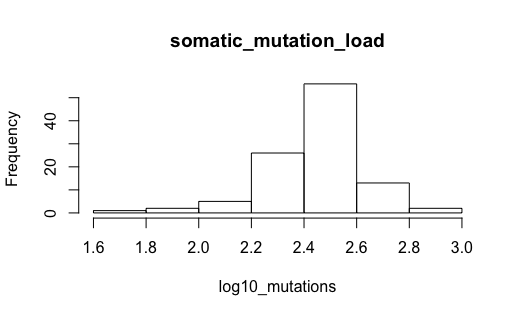
\includegraphics[width=0.8\textwidth]{figures/somatic_mutation_load.png}
\caption{The log$_{10}$ transformed somatic mutation load in 100 patients.}
\label{Somatic_load}
\end{figure}

\section{Japanese cohort eQTL analysis}
\label{eQTL}

A total of 25508 genes were tested, which excludes 180 genes that lack variant information. There were 805 significant eGenes with a FDR threshold below 0.05 after the permutation test. Most of the significant eQTLs for the 805 genes were located close to the transcription start site (TSS) of genes. See figure \ref{TSS} for a location distribution plot. The eQTLs that have the nearest distance(7bp) to TSS sites were chr19\_50344768\_G\_A for gene NAPSB and chr17\_15786625\_A\_G for gene MEIS3P1.

\begin{figure}[h]
\centering
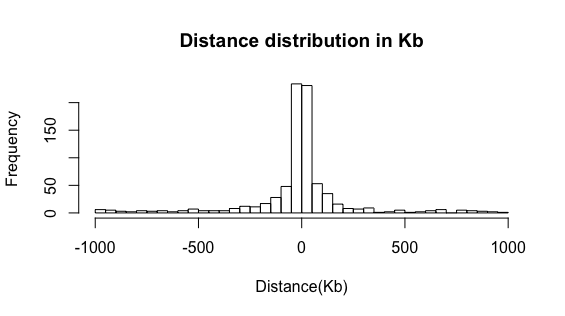
\includegraphics[width=0.8\textwidth]{figures/TSS.png}
\caption{Distance distribution between the most significant cis-eQTL site and the gene TSS site in Kb}
\label{TSS}
\end{figure}

Ranking by q-value of each identified eGenes, the most significant eGenes includes LINC01291(ENSG00000204792.2) which located on chromosome 2,ERAP2(ENSG00000164308.16) which located on chromosome 5, RPS26(ENSG00000197728.9) which located on chromosome 12 and XRRA1(ENSG00000166435.15) which located on chromosome 11. Boxplots in Figure 3.4.2 showed gene expression variation along with those eQTLs.

\begin{figure}
\label{boxplots}
	\centering
	\subfigure[Gene LINC01291 with eQTL rs3771800]{
		\begin{minipage}[b]{0.4\textwidth}
			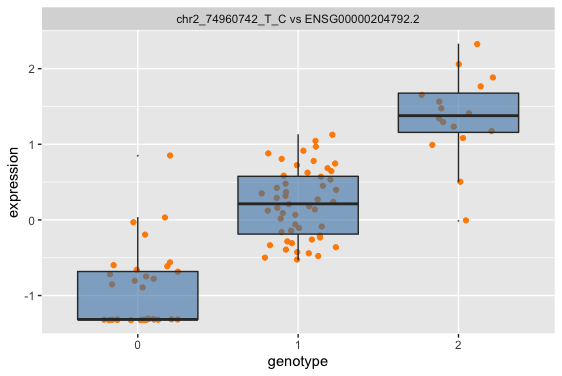
\includegraphics[width=1\textwidth]{figures/LINC01291.png} 
		\end{minipage}
		\label{fig:LINC01291}
	}
    	\subfigure[Gene ERAP2 with eQTL rs2549782]{
    		\begin{minipage}[b]{0.4\textwidth}
   		 	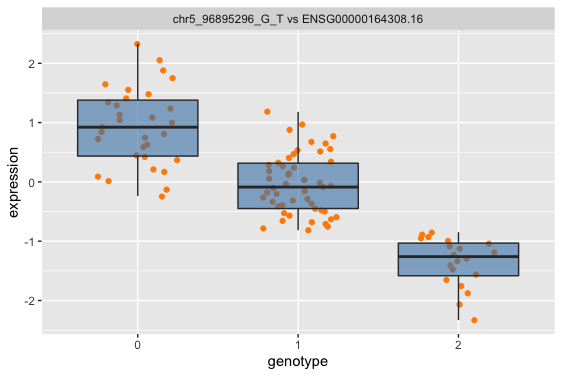
\includegraphics[width=1\textwidth]{figures/ERAP2.png}
    		\end{minipage}
		\label{fig:ERAP2}
    	}
	\\ 
	\subfigure[Gene RSP26 with eQTL rs1131017]{
		\begin{minipage}[b]{0.4\textwidth}
			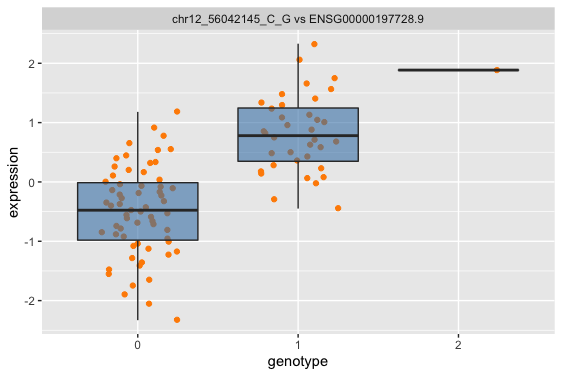
\includegraphics[width=1\textwidth]{figures/RSP26.png} 
		\end{minipage}
		\label{fig:RSP26}
	}
    	\subfigure[Gene XRRA1 with eQTL rs9787775]{
    		\begin{minipage}[b]{0.4\textwidth}
		 	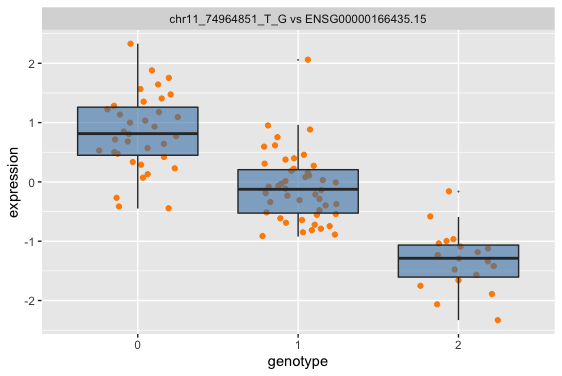
\includegraphics[width=1\textwidth]{figures/XRRA1.png}
    		\end{minipage}
		\label{fig:XRRA1}
    	}
	\caption{The representative eGenes boxplot with corresponding top eQTLs in the Japanese cohort tumor eQTL analysis}
	\label{fig:4-significant}
\end{figure}

In the GTEx published v8 release, whole genome sequencing data from 73 kidney tissues of different individuals were used and 1260 eGenes with FDR < 0.05 were identified. There were 287 eGenes that appeared in both the Japanese cohort and the GTEx V8 release, which accounts for 35.7\% of the total number of identified Japanese cancer eGenes. It is a high proportion of overlap between the eGenes that appear in GTEx databases and the eGenes identified in this study,which proved a credibility of Japanese eQTL analysis. On the other hand, 518 new significant eGenes were discovered for the Japanese cohort.

Among the 518 new eGenes, 162 of them were also identified as having somatic mutations by Mutect2 followed by FilterMutectCalls. There were also 13 significant eGenes that overlapped with highly recurrent somatic mutated genes(at least 5 times): USP24, LRRIQ3, NBPF9, FCRL3, LAMC2, ALMS1, ARFGEF3, DNAH11, PMS2P1, NUP205, RPH3A, TPP2, USP6. The detailed information was showed in table \ref{tab:13eGenes}.
\begin{table}[!ht]
\centering
\caption{13 eGenes that both significant in eQTL analysis and appeared in recurrent mutated genes}
~\\
\label{tab:13eGenes}
\resizebox{15cm}{!}{
\begin{tabular}{llllll}
\toprule
\textbf{gene name}		  & \textbf{gene chr}   &\textbf{variant id} &\textbf{rs id} &\textbf{MAF} &\textbf{qval}                            \\
\toprule
USP24 &chr1 	&chr1\_54679120\_T\_C &rs79149166 & 0.0909091 & 0.0434513\\
\midrule
LRRIQ3	&chr1 &chr1\_74205835\_A\_G	 &rs571848 &0.338384 &2.02546e-09	\\
\midrule
NBPF9 & chr1	&chr1\_149061042\_A\_C &None &0.453125 &1.05064e-12		\\
\midrule
FCRL3 	& chr1 	& chr1\_157698600\_T\_C & 	rs7522061 & 0.373737 &2.40848e-08	\\
\midrule
LAMC2 & chr1	&chr1\_183186347\_C\_A & rs684527 &0.35119 & 0.0194763\\
\midrule
ALMS1& chr2	& chr2\_74380596\_A\_G & None & 0.0104167 & 0.0134938 \\
\midrule
ARFGEF3& chr6	&chr6\_137544329\_T\_A & 	rs203693 &  0.10101 &0.021038\\ 
\midrule
DNAH11 & chr7 &chr7\_21545202\_A\_G & 	rs7781669 &  0.309278 & 1.03004e-15 \\
\midrule
PMS2P1 & chr7 &chr7\_100373690\_T\_C	 & rs2405442 & 0.479798 &5.10579e-06 \\
\midrule
NUP205	 &chr7 &chr7\_134646897\_G\_GGCT	 &None & 0.0121951 & 0.0281559 \\
\midrule
RPH3A & chr12 &chr12\_112875665\_C\_T & rs2891411 &0.444444 & 0.0253587 \\
\midrule
TPP2 & chr13 &chr13\_101692517\_A\_G & rs981073 & 0.0151515 & 0.0181033 \\
\midrule
USP6 & chr17 &chr17\_5461303\_CTTCT\_C & rs199685469 & 0.0159574 & 	0.0186372 \\
\bottomrule
\end{tabular}
}
\end{table}

See figure\ref{Overlap} for a detailed technical description and eGene counts.

\begin{figure}[h]
\centering
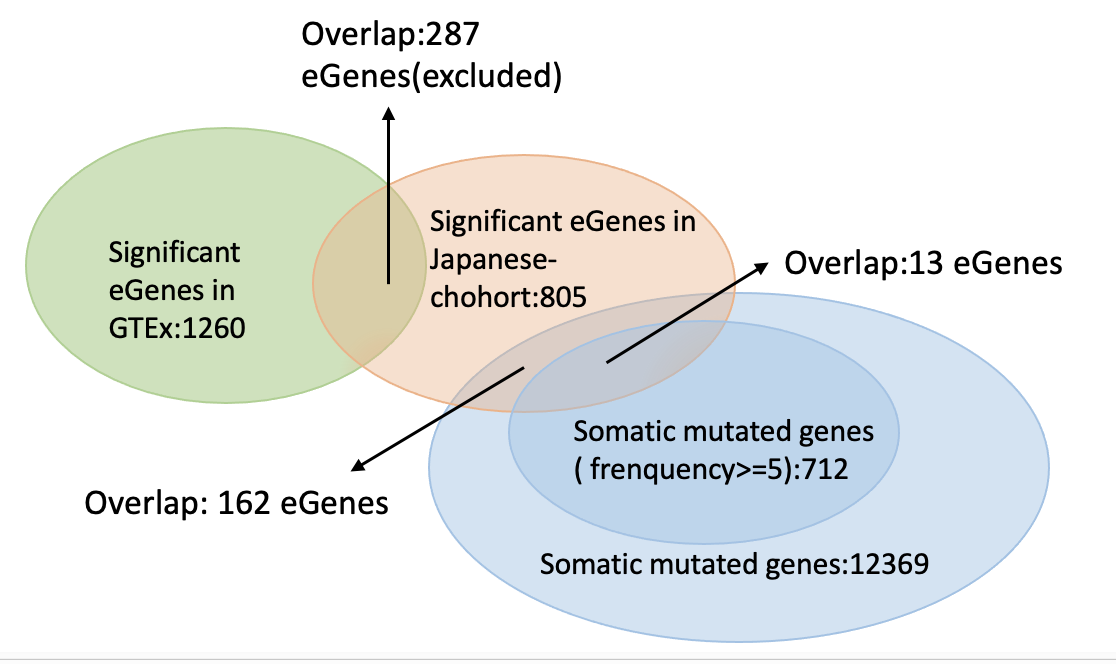
\includegraphics[width=0.8\textwidth]{figures/Overlap.png}
\caption{The study role of finding overlapped eGenes}
\label{Overlap}
\end{figure}

After the variant filtration and association tests, the top eQTLs for each significant eGene was provided in the final eQTL results table, which is available in the appendices\ref{sec:Appendices}. The lowest number of tested variants was 4 sites (for eGene MAS1L and TJP1), and the highest number of tested variants was 1040 sites (for eGene ZNF468). Besides, all the significant gene-SNP pairs were provided in another table in the appendices \ref{sec:Appendices}.



\section{Enrichr results}
The 13 eGenes and 162 eGenes described in section \ref{eQTL} were submitted to Enrichr Gene set enrichment analysis (GSEA). For the 13 highly recurrent mutated eGenes, the most significantly enriched pathway was Extracellular matrix(ECM) receptor interaction (p-value = 0.05) based on KEGG 2019 human. The gene LAMC2 was enriched in this pathway. For the 162 eGenes, the most significantly enriched pathway was Homologous recombination(HR)(p-value = 0.04).The genes BABAM1 and RAD52 were enriched in this pathway.


\chapter{Discussion}

\section{Technical methods discussion}

The development of cancer is a sophisticated process. In the study of cancer mechanisms, driver mutations mentioned in section \ref{subsec:Variants type appeared in cancer tissues} are important for discovering oncogenic pathways. In this study, a new study flow was designed specifically for the existing sequencing data. Firstly, a direct mutation-calling workflow was applied to the tumor samples. Technically, all the variants that appeared in tumor samples and were different from the reference genome are able to be called. After a systematic variants quality control and filtration, the passed variants site and genotypes were tested with tumor sample's gene expression. The idea of this workflow is based on normal eQTL analysis that tests the association between normal sample genotypes and normal sample expression. This type of regular eQTL analysis is based on the absolute expression value change of the sample. For this reason, the absolute gene expression change should perform the association test with absolute genotype change. Usually, the genotypes of samples have a two-stage change. First, the normal samples always have some different genotypes with the reference genome. Then, the tumor samples always have different genotypes from normal samples. Consequently, the genotype variation in either normal-reference pair or tumor-reference pair is all absolute genotype changes. Conversely, the genotypes called between tumor and normal samples were relative genotypes change. This might cause a significant loss in the eQTL test. 

Based on the former illustration, the association test was performed between tumor sample genotypes and tumor gene expressions. The filtering steps used some common principles and thresholds that apply in population genomics, like minor allele frequencies and missingness, to ensure the quality of the test. Most variant sites were filtered because of >25\% genotype missingness. This is to keep the rest sites have enough confident genotype information between individuals for an eQTL analysis. Meanwhile, the tumor samples with matched normal samples provided the possibility to call somatic mutations separately. After the filtration, the distribution of somatic mutation load is similar to another research by Liu et al.\cite{liu_association_2018}. The somatic mutations were used to compare with the significant eGenes detected before and find the recurrently mutated eGenes.

\section{Results discussion}

\subsection{Mutation calling results}

The mutation calling result of tumor tissue using HaplotypeCaller implicated that most mutations are not harmful for gene function. A lot of them fall into the intron region or other non-protein-coding regions. There were above 99.6\% of mutations that did not change the type of coded amino acids. In comparison, the Mutect2 algorithms combined normal tissues and tumor tissues to find somatic mutations, and the proportion of putative 'HIGH' impact mutations was higher than HaplotypeCaller's result. Meanwhile, the proportion of missense mutations was much higher than nonsense mutations, which suggests that mutations that happen during cancer cell development have higher possibilities to change the gene-coded amino acid type.

Previous known key ccRCC gene VHL (von Hippel Lindau gene) have a sum of 54 times mutation in the Mutect2 somatic calling results. The mutated VHL gene that lost the functions will cause a high level of HIFα factor. The HIFα factor controls multiple downstream gene expression, such as VEGF, PDGF and TGFα\cite{clark_role_2009}. The VEGF and PDGF family genes have also appeared in somatic mutation results. In the study by yang et al.\cite{yang_gene_2017}, the VHL gene has a significant association with differential expressed gene modules. In this study, the most significant eQTL site for VHL gene was a deletion (ATCT > A) with rs id rs5030648, which has a q value of 0.569 but did not achieve a significant q value below 0.05. Therefore, the VHL gene might has a hidden comprehensive disease-causing mechanism that different with the direct mRNA expression decrease. 

\subsection{The possible mechanism of identified significant eGenes results}

The identified significant eGenes have more than 35\% overlap with significant eGenes in GTEx kidney V8 release. These eGenes were significantly being controlled in two different cohorts of kidney tissue, one of which contained healthy tissue and the other contained cancer tissue. Often, it will be acceptable to have a relatively small overlap between two results, even if they all originate from kidney tissue. The population composition of these two cohorts is different, so the two cohorts might originally carry their own feature SNPs. Furthermore, even this study has mostly tried to replicate the same workflows of the GTEx database, but the different sequencing methods, the minor changes in details in workflows and different sample size could all affect the final eQTL results. Considering these variable factors, the overlapped eGenes still account for more than 35\% of total eGenes in this study. This high proportion of overlap suggests a high similarity in gene expression regulation between different kidney tissues. This kind of similarity might because of the same potential germline variants in both cohorts that controls the corresponding gene expression. Even tumor cells have changed a lot in gene expression, tumor cells will keep some extent of similarity with normal cells, especially for key genes such as housekeeping genes. These genes expression might controlled by specific genetic loci, that both identified in tumor cells and normal cells. 

On the other hand, significant gene regulation changes also appeared in cancer patients of the Japanese cohort. This change might be caused partially by population differences, but more likely caused by tumor-specific variation. 

The significant eGenes have shown a certain extent of relationships with ccRCC disease mechanisms. Among the four most significant eGenes, some showed relationships with ccRCC based on previous publications, but others did not. The gene LINC01291 is a long intergenic non-protein coding RNA gene, which has been reported with an impact that promotes the aggressive properties of melanoma. The boxplot(a) demonstrates the increase in expression of LINC01291 when the mutation occurred. It competes with specific miRNAs and increases the expression level of IGF-1R (insulin-like growth factor-1 receptor)\cite{wu_long_2021}. The insulin-like growth factor (IGF-1) pathway is also an important pathway in the development of ccRCC. The higher expression of IGF-1R leads to a higher risk of death for ccRCC patients\cite{tracz_insulin-like_2016}. The lncRNAs have been emphasized in the Introduction section for their important regulatory functions. Except LINC01291, another lncRNA named TRIM52-AS1 was discovered to function as a tumor suppressor gene for ccRCC according to the research by Liu et al.\cite{liu_downregulation_2016}. The TRIM52-AS1 is down-regulated in renal cell carcinoma (RCC) tissues, which suggests the low expression value of TRIM52-AS1 might lose its function as a tumor suppressor. TRIM52-AS1 was also identified as one of the eGenes in the Japanese cohort. The most significant eQTL site is chr5\_181260427\_CTCT\_C with dbSNP id rs200454506. Based on the boxplot drawn by the provided script, the happened deletion will cause a decrease in expression value, which might lead to tumor development. Notably, the LncRNA gene family has been identified not only as significant eGenes but also as highest recurrently mutated sites(BAGE2), which indicates the importance of lncRNA in gene expression regulation of ccRCC.

The second identified significant eGene ranked by q-value is ERAP2 (endoplasmic reticulum aminopeptidase 2). ERAP2 encodes multifunctional enzymes that have a great biological function when cell-generating major histocompatibility complex (MHC) class I binding peptides\cite{compagnone_regulation_2019}. This process might influence tumor immunogenicity. Research about anti-PD1 response in ccRCC \cite{au_determinants_2021}have identified ERAP2 mutation as a signature gene related to defective antigen presentation. The boxplot(b) in Figure \ref{boxplots} showed that the mutation of ERAP2 decreased the gene expression level so that potentially decreased the level of enzymes. 

Some significant eGenes have not been reported in ccRCC research before. The gene RPS26 (Ribosomal protein S26) is a disease-related gene, and the mutation of RPS26 usually causes Diamond-Blackfan Anemia 10 (DBA10)\cite{doherty_ribosomal_2010}. This gene functions in pre-rRNA processing but no evidence showed its relation with kidney cancer in previous studies. Notably, the RPS26 protein has been implicated in regulating the p53 response to DNA damage\cite{cui_ribosomal_2014}. The p53 protein mostly has great impacts on different cancers, which suggests RPS26 as a newly discovered key gene for ccRCC. The gene XRRA1 (X-Ray Radiation Resistance Associated 1) is also a gene related to DNA damage repair. A few works of literature mentioned that it might be related to cancer development, such as the study by Wang et al.(2017)\cite{wang_xrra1_2017}, that showed XRRA1 targets ATM/CHK1/2-Mediated DNA Repair in Colorectal Cancer.

\subsection{The possible mechanism of identified 13 recurrently mutated eGenes}

All the 13 eGenes are somatically mutated at a frequency of at least five times in all the 100 patients. The Ubiquitin Specific Peptidase 24 (USP24) and Ubiquitin-specific protease 6 (USP6) are belongs to the same family of ubiquitin-specific peptidases (USPs). USPs play a significant role in a wide variety of diseases, and a growing number of studies reveal that USPs are crucial for cancer progression. Specifically, USP24 blocks the progression of the cell cycle from metaphase to anaphase, resulting in cell cycle arrest. It is a novel tumor suppressor identified by Bedekovics et al.(2021)\cite{bedekovics_usp24_2021}. USP6 is involved in activating the NFκB pathway, thereby positively influencing tumorigenesis\cite{young_role_2019}. Additionaly, USP6 is a key mutated gene in the VHL-negative ccRCC patients\cite{tan_establishment_2013}. Thus, the corresponding eQTLs for these two eGenes that were identified in this study have high potential to play the role as driver mutations in ccRCC.

The Leucine Rich Repeats And IQ Motif Containing 3 (LRRIQ3) is a protein coding gene. It is down-regulated in a number of cancers based on the tissue expression data from The Human Protein Atlas. Laminin Subunit Gamma 2 (LAMC2) encodes a part of protein called laminin 5. Laminins are a group of proteins that regulate cell growth, cell motility and cell adhesion. The silencing of LAMC2 will inhibit angiogenesis, which is a crutial driver in ccRCC pathogenesis\cite{pei_silencing_2019}\cite{seles_long_2020}. The mutation of ALMS1 Centrosome And Basal Body Associated Protein (ALMS1) causes Alstrom syndrome which is a rare genetic disorder, but the encoded protein has multiple functions such as maintaining the cohesion and composition of centrosomes, organizing the actin cytoskeleton\cite{hearn_alms1_2019} and regulating the TGF-β signaling pathway\cite{alvarez-satta_alms1_2021}. The Nucleoporin 205 (NUP205) have been identified to be drivers of lung cancer\cite{fujitomo_critical_2012}. Tripeptidyl-peptidase 2 (TPP2) has been discovered to be significantly up-regulated in oral squamous cell carcinoma derived cells. Also, the overexpression of TPP2 leads to accelerated cell growth and resistance to apoptosis\cite{tomkinson_tripeptidyl-peptidase_2019}. The Neuroblastoma Breakpoint Family Member 9 (NBPF9), Fc receptor-like protein 3 (FCRL3), ARFGEF Family Member 3 (ARFGEF3), Dynein Axonemal Heavy Chain 11 (DNAH11)and Rabphilin 3A (RPH3A) are the genes that has not been reported as cancer related genes before. PMS2P1 is a pseudogene so we didn't discuss it here. 

\subsection{The discussion about pathways enriched by Enrichr}
The Enrichr results have given two important potential disease-related pathways: ECM-receptor interaction and Homologous recombination. ECM-receptor interaction pathway is a cancer-related pathway. The role of ECM has been proved in different types of cancers, such as prostate cancer, colorectal cancer, and breast cancer\cite{bao_transcriptome_2019}. Homologous recombination(HR) has been proved to be highly related to ccRCC. SETD2, one of recurrently mutated genes, has been proved to affect the efficiency of homologous recombination repair in ccRCC through the loss-of-function mutations\cite{kanu_setd2_2015}. 

\subsection{Conclusion}

As a conclusion, this study has provided a database of newly identified significant eGenes and eQTLs of the Japanese ccRCC patient cohort. The database provides a reference for future analyses. Several potential key genes have also been identified. The LINC01291, for instance, is a gene with a high significance that is related to the development of ccRCC. We also derived a list of recurrently mutated significant eGenes based on the results of somatic mutation calling and eQTL analysis. Some of these have just been discovered, and others have already been proven to be closely related to ccRCC and could be potential drug targets, such as USP24 and USP6. It is more likely these 13 eGenes will serve as driver genes due to the presence of somatic mutations.  In summary, this study investigated tumor-specific eGenes and eQTL sites in comparison to healthy kidney eGenes, and achieved a combined analysis through the detection of somatic mutations within tumor cells to identify recurrently mutated eGenes as potential driver genes for ccRCC.

\section{Delimitations}

This project has used the whole-exome sequencing data as genotype data, so only variants located inside genes or near genes were able to be detected. Since this project focused on cis-eQTL mapping, the whole-exome sequencing should not cause a large impact in principle. In the variants filtering step, several samples have a relatively high missing genotypes rate based on Plink and SnpEff, but were not excluded in the downstream analysis.  In this way, a complete cohort of 100 patients was kept. But some missing genotypes inside those individuals have been kept in the variant sites. After generating the tumor-specific eQTLs table, the downstream analysis changed to focus on gene-level (eGenes)rather than mutation level. As a result, future work is needed to complete the information on eQTL level.
\chapter{Future work}

The future work can be summarized as following points:\\
1) Get the data on DNA methylation and tumor somatic copy number variations. Based on the normal sample's genotype calling, perform a germline-based eQTL analysis of tumor expression, which considered the DNA methylation and tumor somatic copy number variations separately. This method might be able to give more information on the germline level. The potential inherited risk loci might be found.\\
2) Get a larger cohort to call somatic mutations intensively in order to get enough genotypes at the same mutated loci (around 50bp). Perform an eQTL analysis purely based on somatic mutations to reveal more driver mutations in ccRCC development. \\
3) Build online websites to visualize all the eQTL results, including information searching and figure generation based on queries.\\
4) Perform more pathway analysis and survival analysis based on existing eQTL results.

\chapter{Ethical reflection}

In this study, the patient’s original identity information was kept confidential, and the researchers could only get metadata about the age, gender, cancer condition, and sampling status. In addition, this research is all based on computer data analysis, so it does not involve any ethical issues.
The study has no competing financial interests.




% \include{content}

\newpage
\addcontentsline{toc}{chapter}{References}
\printbibliography


\newpage
\appendix
\newpage
\etocdepthtag.toc{mtappendix}
\etocsettagdepth{mtchapter}{none}
\etocsettagdepth{mtappendix}{subsection}
%\etoctocstyle{1}{Appendix - Contents}
%\tableofcontents
%\newpage
\chapter{Github repository}
\label{sec:Appendices}
All the appended files were provided in a Github repository \href{https://github.com/xiyasong/Degree-project}{https://github.com/xiyasong/Degree-project}.

All the scripts that used for DNA-sequencing analysis, RNA-sequencing analysis and downstream analysis were provided in attached Github address,folder 'Scripts'. The final results of eQTL mapping results were also available in folder 'Results'. Additional data files were available in the corresponding  folders. Detailed information is provided in the README file.
\newpage
% This is the last page of the document
\thispagestyle{empty}
\AddToShipoutPictureBG*{%]
    \AtPageLowerLeft{%
        
\includegraphics[width=1.0\paperwidth]{setup/img/kth-footer.png}
    }%
}

\PlaceText{20mm}{282mm}{\color{white}\fontsize{12}{0}\sffamily www.kth.se }


\end{document}